Navigace v dokumentu je realizována v podobě navigačního podokna, které si uživatel může v pracovním prostředí Atomu
zobrazit s pomocí příkazu \mintinline{text}{wootom:toggleNavigation}, klávesové zkratky (ve výchozím nastavení \textit
{Alt + N}), položky \uv{Wootom: Toggle Navigation} v kontextovém menu nebo podpoložky \uv{Toggle Navigation} položky
\uv{Wootom} v hlavním menu Atomu.

\begin{sloppypar}
Po zobrazení navigačního podokna (které se nejprve zobrazí napravo podokna editoru aktuálně otevřeného souboru; uživatel
si jej případně může přemístit) je aktuálně otevřený soubor rozparsován do AST. Z AST je pak získán seznam všech vrcholů,
které reprezentují části dokumentu a seznam všech vrcholů, které mají v meta-datech neprázdnou položku \mintinline{text}
{label}.
\end{sloppypar}

Ze seznamu vrcholů částí dokumentu je pak vytvořena jednoduchá stromová struktura reflektující úrovně konkrétních částí
(toto je potřeba provést, protože vytvořený AST části nevnořuje podle úrovně) z té je vytvořen číslovaný víceúrovňový
HTML seznam obsahující nadpisy daných částí. Nadpisy jsou přeloženy do HTML s pomocí volání \mintinline{text}
{RenderingManager#render}, čímž je zajištěno i zobrazení případných vnitřních prostředí. Seznam vrcholů AST se značkou
je abecedně seřazen a poté je z něj vytvořen jednoduchý nečíslovaný HTML seznam, obsahující název značky, druh vrcholu
(případě také jeho variantu) a jeho počáteční řádek. Všem položkám obou HTML seznamů je přidán \textit{event listener}
pro událost \textit{click}, který při kliknutí na položku seznamu skočí v editoru aktuálně otevřeného souboru na pozici
začátku daného prvku.

Tyto HTML seznamy jsou vloženy do navigačního podokna a pro přehlednost uvedeny nadpisy. Mezi nadpis a seznam je pak
vždy vloženo textové pole, s jehož pomocí může uživatel v seznamu vyhledávat relevantní položky. Vyhledávání je spuštěno
při libovolném uživatelském vstupu; pokud uživatel svůj dotaz vymaže, je vyhledávání zrušeno. Při vyhledávání v seznamu
částí dokumentu je vyhledáváno v textech nadpisů částí a výsledný seznam je zploštěn (už není víceúrovňový). Při
vyhledávání v seznamu značek je vyhledáváno pouze v názvech značek. Seznam výsledků vyhledávání je seřazen od největší
shody po nejnižší shodu.

Pro vyhledávání byla využita knihovna Fuse.js, která umožňuje fuzzy vyhledávání, kdy dotaz uživatele nemusí přesně
odpovídat vyhledávanému textu (dle dokumentace \cite{fuse-docs} knihovna využívá modifikovanou verzi algoritmu Bitap).
Tato knihovna byla dále vybrána díky její přehledné dokumentaci, dostupnosti TypeScript \textit{types}, permisivní
open-source licenci a velké popularitě (mezi 1,5 miliony a 3 miliony týdenních stažení z npm \cite{npm} za poslední
rok). Knihovna dále dle \cite{fuse-docs} umožňuje upravit mnoho různých parametrů vyhledávání, takže je v případném
budoucím vývoji možno například upravit mezi, které musí shoda dotazu a vyhledávaného textu dosáhnout.

Na obrázku \ref{navigace-pkm} je pro ilustraci zobrazeno okno Atomu s otevřeným souborem zdroje studijního textu k
BI-PKM na levé straně a jeho navigačním podoknem na pravé straně.

\begin{figure}\centering
    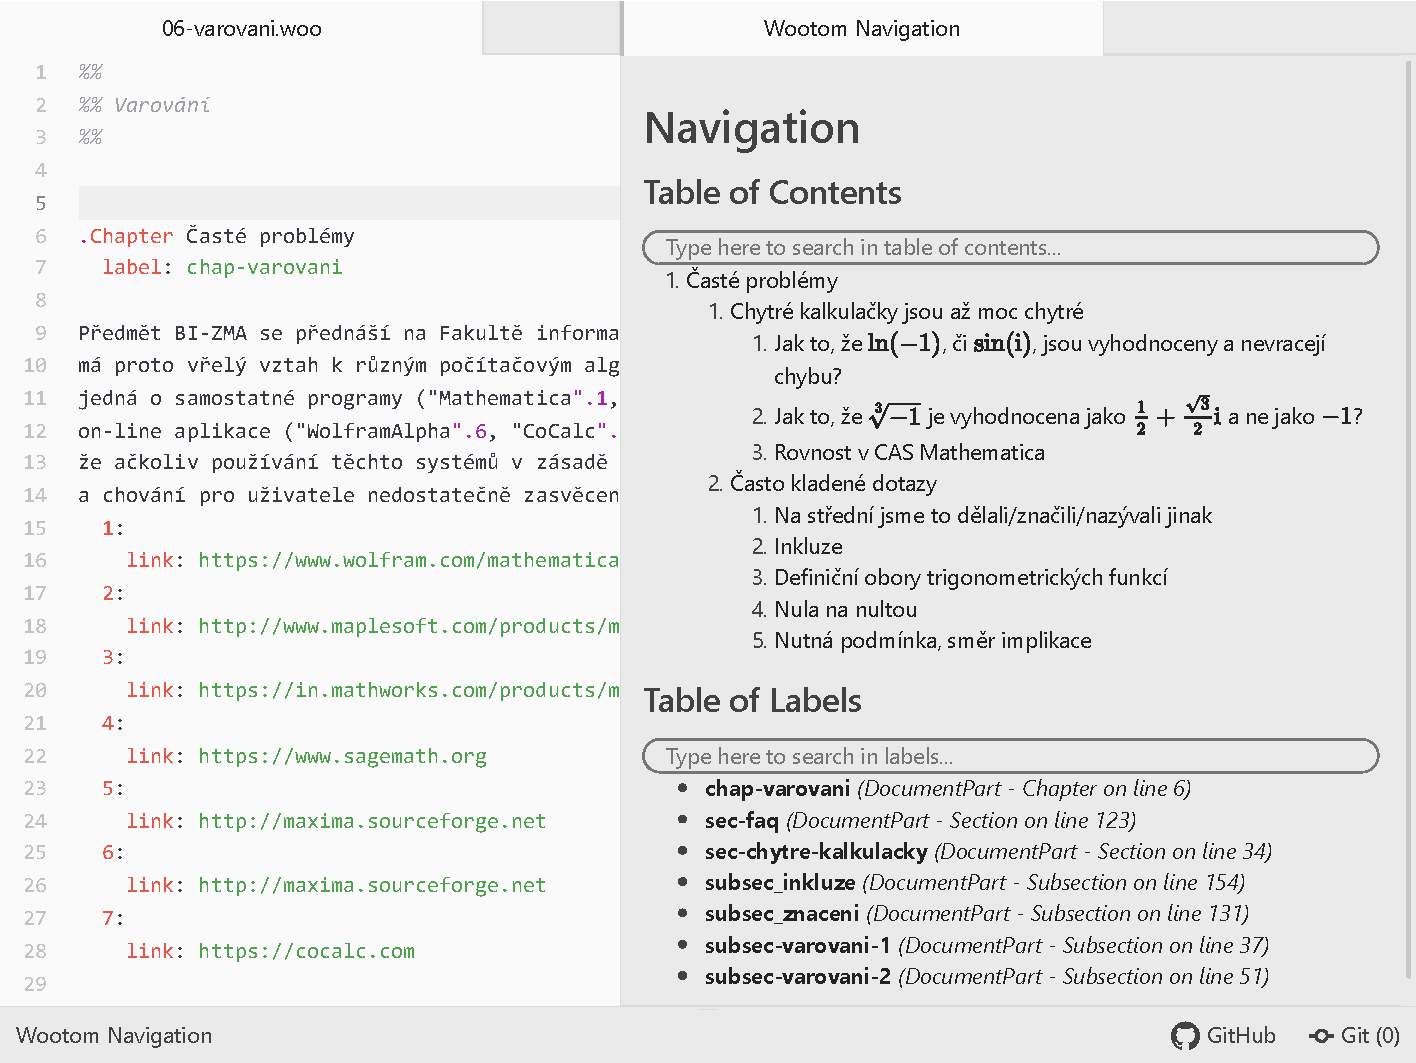
\includegraphics[width=1.0\textwidth]{content/realizace/navigace-pkm}
 	\caption[Navigace v dokumentu]{Navigační podokno u otevřeného souboru zdroje studijního textu k BI-PKM \cite{pkm}}
    \label{navigace-pkm}
\end{figure}

Tímto byly realizovány funkční požadavky \textbf{F6} až \textbf{F10}. Implementaci by bylo dále možno vylepšit například
o zobrazení přehledu částí a značek v celém dokumentu (nikoliv v pouze aktuálně otevřeném souboru).
